\begin{minipage}{0.3\textwidth}
\section*{R-A*mbush}

\begin{itemize}
\item Getting agents to perform A$^*$mbush from their
starting point can be disadvantageous, since they can
take unnecessarily longer routes.

\item R-A$^*$mbush is an A$^∗$mbush modification that
performs A$^∗$ until the agent gets inside a fixed radius
$R$ around the goal point.

\item Once at this stage, the agent starts performing A$^∗$mbush.

\end{itemize}

\begin{center}
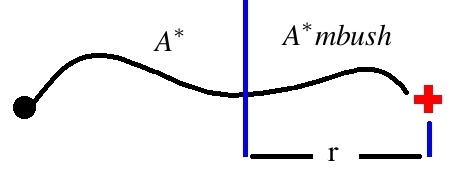
\includegraphics[width=0.8\textwidth]{figures/rambush.jpg}
\end{center}
\end{minipage}